\documentclass[tikz,border=10pt]{standalone}
\usetikzlibrary{angles,quotes}
\begin{document}
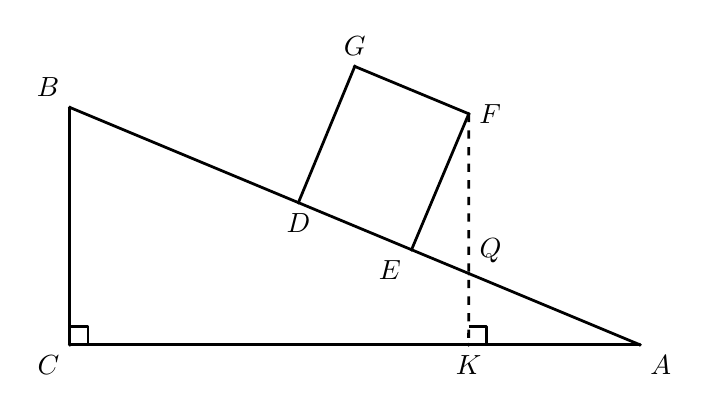
\begin{tikzpicture}[line width=1.0pt, line join=round, font=\fontsize{10}{12}\selectfont]
\coordinate (A) at (3.618,-1.762);
\coordinate (B) at (-3.621,1.252);
\coordinate (C) at (-3.621,-1.762);
\coordinate (D) at (-0.719,0.043);
\coordinate (E) at (0.718,-0.555);
\coordinate (G) at (-0.003,1.773);
\coordinate (K) at (1.443,-1.762);
\coordinate (Q) at (1.447,-0.858);











\coordinate (F) at (1.445,1.171);


\draw (B) -- (C) -- (K) -- (A);
\draw (B) -- (D) -- (E) -- (Q) -- (A);


\draw (G) -- (D);
\draw (F) -- (E);
\draw (G) -- (F);


\draw[dashed] (F) -- (K);


\draw pic[draw, angle radius=0.230cm] {right angle=A--C--B};


\draw (1.443,-1.532) -- (1.673,-1.532) -- (1.673,-1.762);

\foreach \p in {A,B,C,D,E,F,G,K,Q}
  \fill (\p) circle (0.025);


\node[above left] at (B) {$B$};
\node[above] at (G) {$G$};
\node[right] at (F) {$F$};
\node[below] at (D) {$D$};
\node[below left] at (E) {$E$};
\node[below left] at (C) {$C$};
\node[below right] at (A) {$A$};
\node[below] at (K) {$K$};
\node[above right] at (Q) {$Q$};
\end{tikzpicture}
\end{document}